\headline{{\textbf{\Large\sffamily Potting Shed Gossip:}}\\
          {\textbf{\large\sffamily The Great (Roots) Escape}}}
\label{2025-03-gossip}
\noindent
This month, \textbf{Tina Todd} has got us all talking with a fascinating \href{https://www.facebook.com/share/r/19yJ96N9Pz/}{video} she shared on our club's WhatsApp channel.
\textbf{Ever dreamt of thickening your bonsai's trunk without the hassle of planting it in the ground?}
Well, grab a bucket---literally!

The video showcases a rather genius (and slightly rebellious) technique: simply take a deep bucket, half\--fill it with soil, and plop your potted bonsai right in the middle.
Then, pile in more soil until it swallows up the pot, leaving only the trunk exposed---like a bonsai hot tub, but for growth, not relaxation!
In just a couple of months (and, let's be honest, some serious tropical humidity judging by the background), the roots burst out of the original pot, stretching into their newfound kingdom restoring the plant's vigour and thickening the trunk at an astonishing rate.
Once it's bulked up, you simply unearth your tree, trim the excess roots, and restore it to its former bonsai glory---none the wiser!

A simple, sneaky, and surprisingly effective trick---who knew bonsai could be such escape artists?

Got a bonsai\--related rumour, quirky story, or fun fact?

\noindent
Share it with us for the next edition of \textit{Potting Shed Gossip!}

%\vfill
\begin{window}[%
    2,l,%
    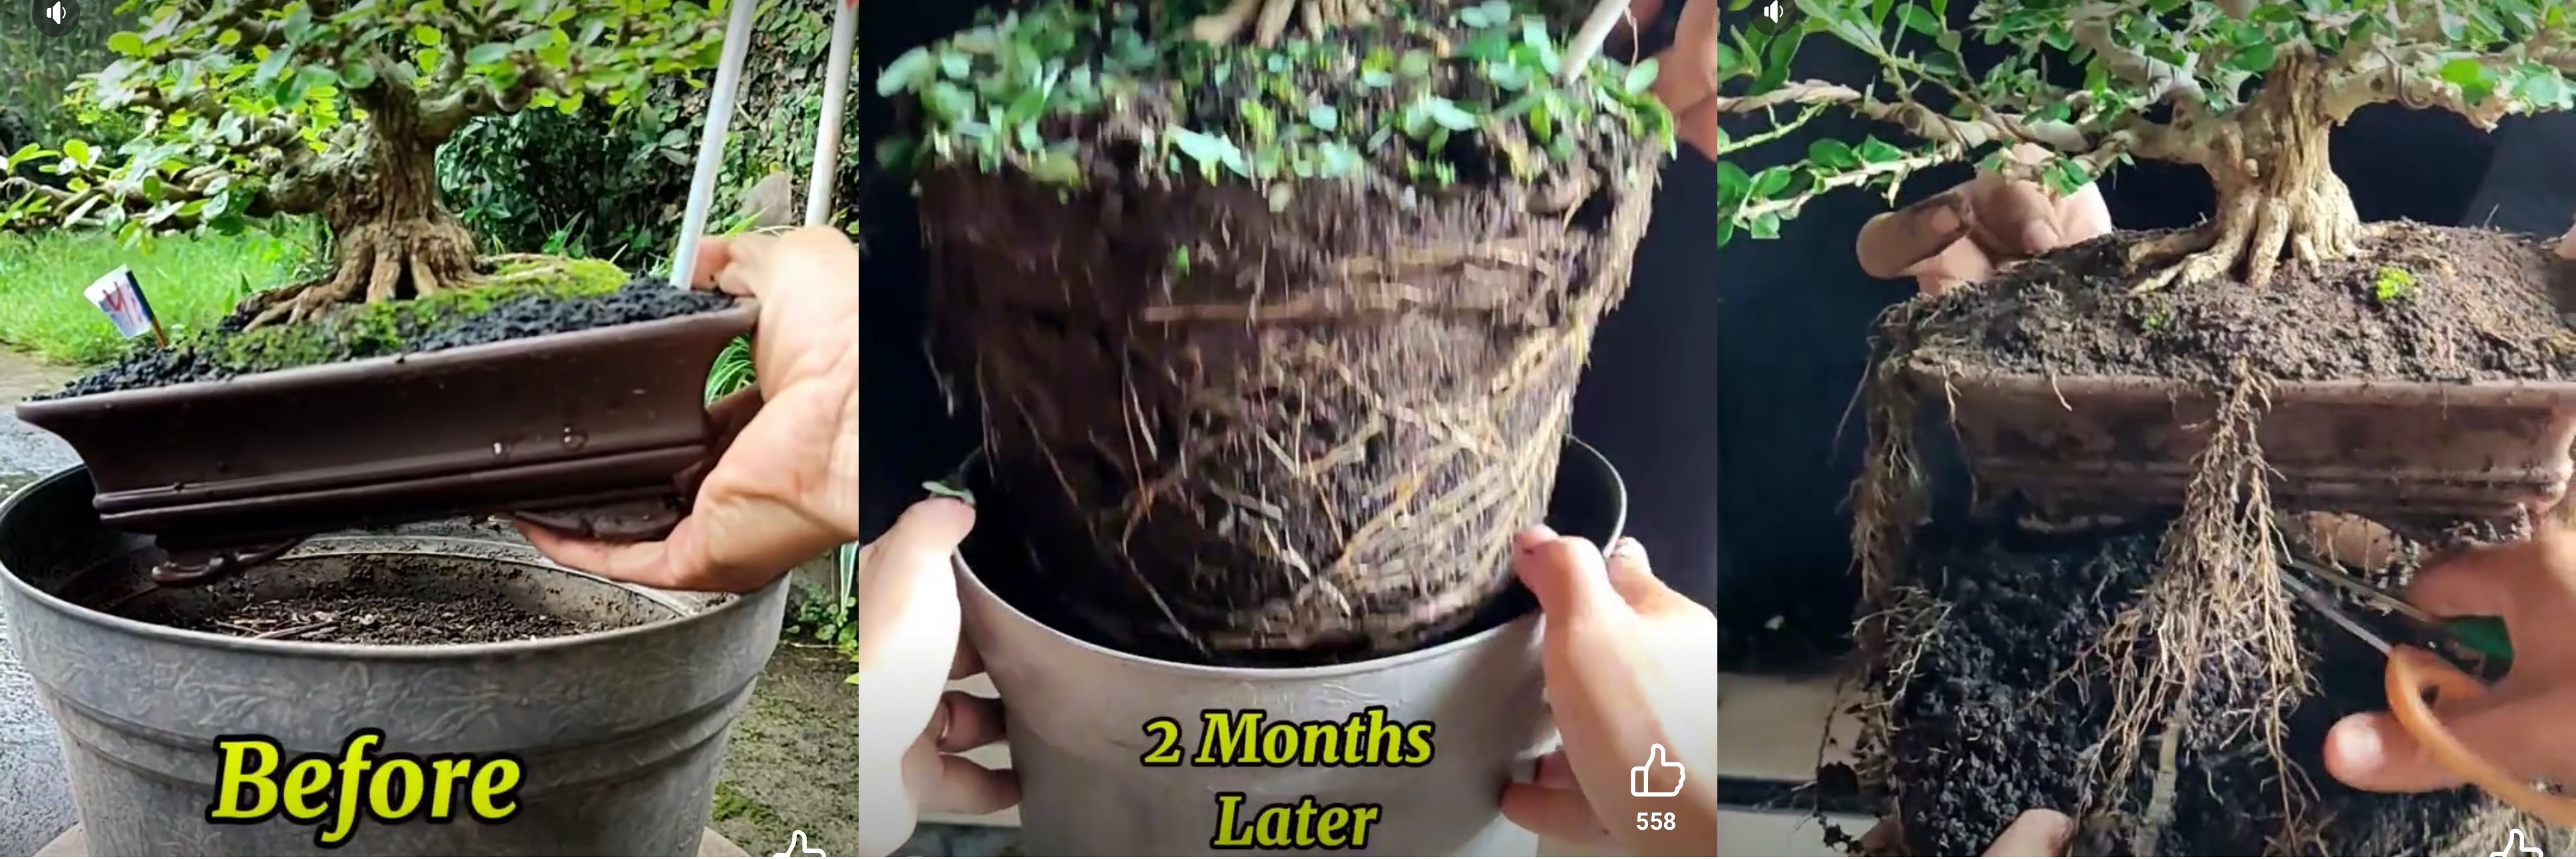
\includegraphics[width=1.0\columnwidth]{2025_03/res/gossip},%
    \centerline{\emph{Key moments from the video showcasing the method.}}%
]
\end{window}
\closearticle
%
%\vfill
%\begin{center}
%    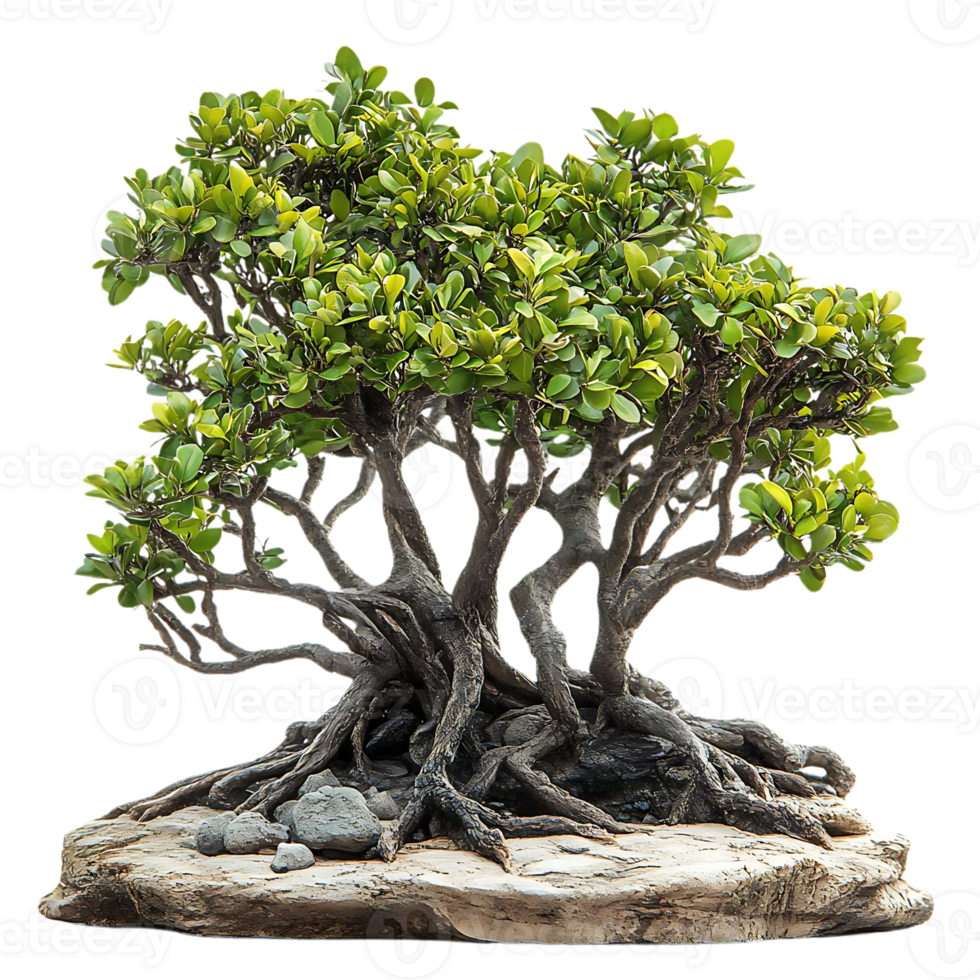
\includegraphics[width=0.8\columnwidth]{res/filler_b}
%\end{center}
%\columnbreak
